\documentclass[titlepage]{report}
\usepackage[spanish]{babel} % espanol
\usepackage[latin1]{inputenc} % acentos sin codigo
\usepackage{graphicx} % graficos
\begin{document}
\begin{titlepage}

\begin{center}
\vspace*{-1in}
\begin{figure}[htb]
\begin{center}

\includegraphics[width=8cm]{4344.png} 
\end{center}
\end{figure}

Universidad Aut\'{o}onoma de San Luis Potos\'{i}\\
\vspace*{0.15in}
Facultad de Ingenier\'{i}a\\
\vspace*{0.15in}
\'{A}rea de Ciencias de la Computci\'{o}n\\
\vspace*{0.6in}
\begin{Large}
 Alumno:\\
\end{Large}
\vspace*{0.15in}
Braulio Alejandro Garc\'{i}a Rivera\\
\vspace*{0.6in}
\begin{large}
Titulo:\\
\end{large}
\vspace*{0.2in}
\begin{Large}
\textbf{Maual de Usuario} \\
\end{Large}
\vspace*{0.3in}
\rule{80mm}{0.1mm}\\
\vspace*{0.1in}
\begin{large}
Profesor: \\
Maria Teresa Lucio Gil \\
\end{large}
\end{center}
\end{titlepage}
\chapter*{Interfaz}
\begin{center}
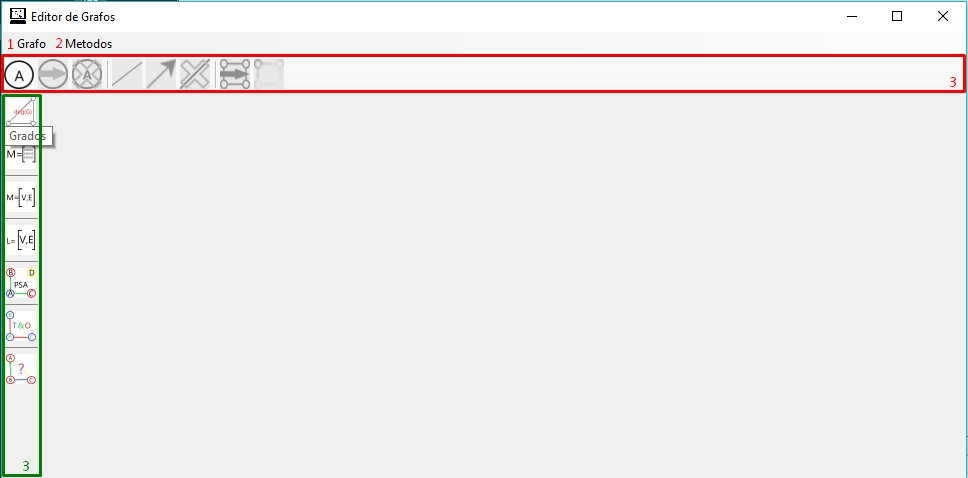
\includegraphics[scale=.60]{Imagen/1.jpg} 
\end{center}
\begin{description}
\item[1:] Menu de operaciones del grafo
\item[2:] Menu de Metodos del grafo
\item[3:] Tool bar de operaciones del grafo
\item[4:] Toolbar de Metodoos de grafo
\end{description}

\chapter*{Operaciones de grafo}
\begin{center}
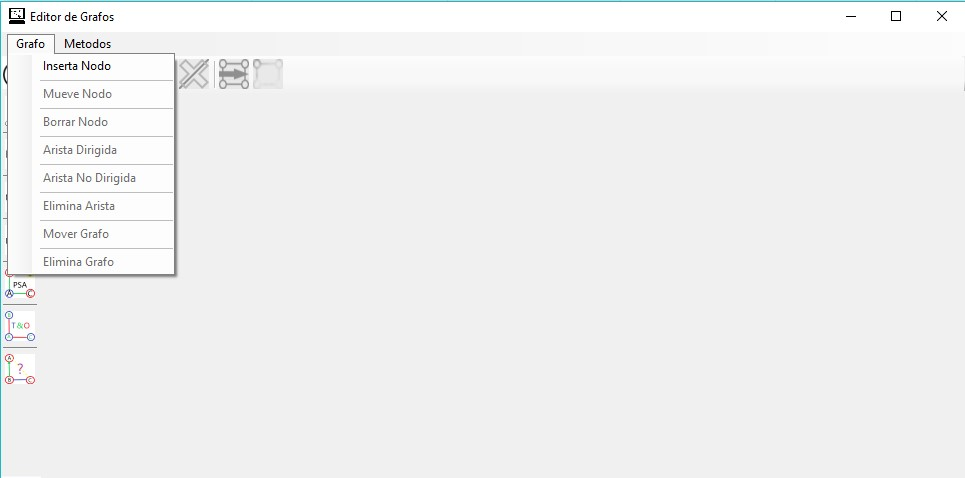
\includegraphics[scale=.60]{Imagen/2.jpg} 
\end{center}
\begin{center}
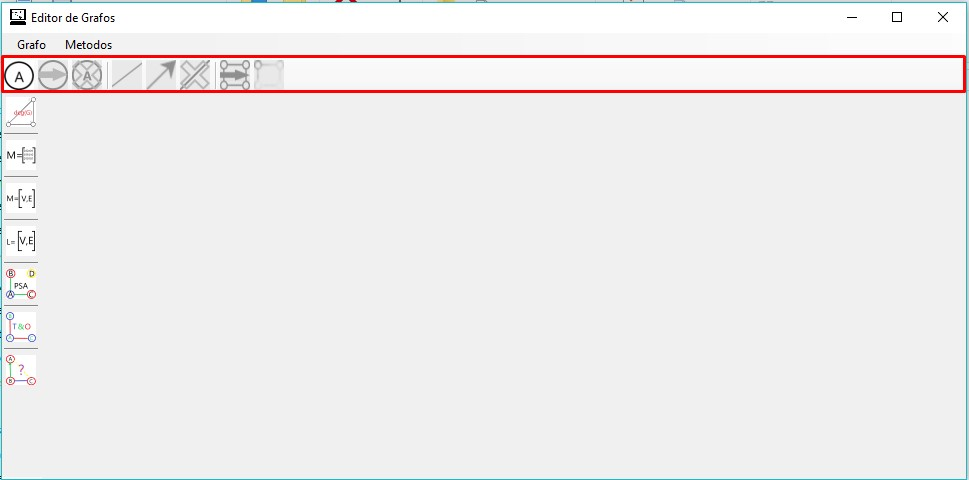
\includegraphics[scale=.60]{Imagen/3.jpg} 
\end{center}
\begin{description}
\item[Insertar Nodo:] Selecciona la opci\'{o}n de insertar nodos al dar click
\item[Mover Nodo:] Selecciona la opci\'{o}n de mover nodos al dar click en uno
\item[Eliminar nodo:] Selecciona la opci\'{o}n de eliminar un nodo al dar click en uno
\item[Arista dirigida:] Selecciona la opci\'{o}n de Eliminar una arista dirigida al dar clic en un nodo arrastrar la arista y soltarlo en otro (al insertar una arista dirigida se inhabilita las opciones del grafo no dirigido)
\item[Arista no dirigida:] Selecciona la opci\'{o}n de Eliminar una arista no dirigida al dar clic en un nodo arrastrar la arista y soltarlo en otro (al insertar una arista no dirigida se inhabilita las opciones del grafo dirigido)
\item[Eliminar arista:] Selecciona la opci\'{o}n de eliminar una arista al dar click en una
\item[Mover Grafo:] Selecciona la opci\'{o}n de mover el grafo al dar click en un nodo del grafo y arrastrarlo a la zona deseada
\item[Eliminar Grafo:] Elimina todo el grafo
\end{description}
\chapter*{Metodos del grafo}
Estos son 2 men\'{u}s uno para cada tipo de grafo y un toolbar que sirve para ambos permite hacer llamadas a los m\'{e}todos del grafo que est\'{e}en programados, los  men\'{u}s son mutuamente excluyentes entre si es decir que cuando est\'{a} habilitado uno el otro esta inhabilitado
\begin{center}
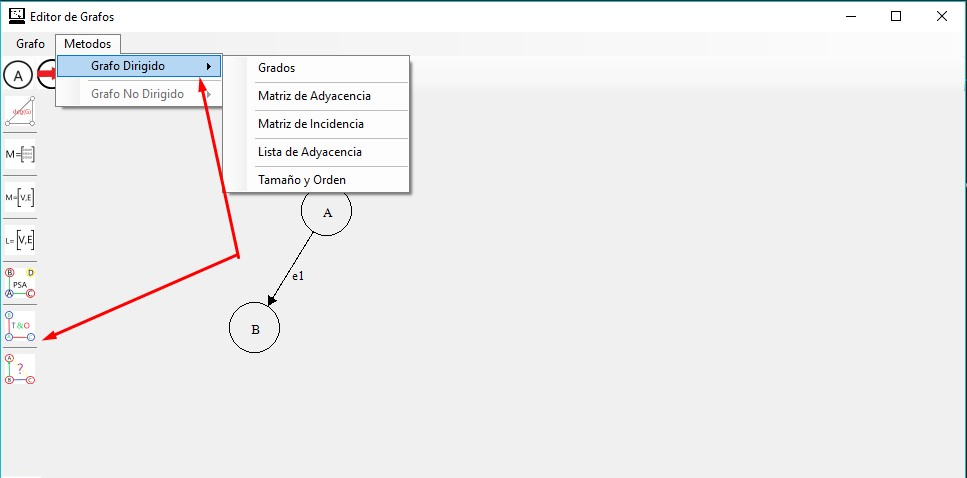
\includegraphics[scale=.60]{Imagen/4.jpg} 
\end{center}
\begin{center}
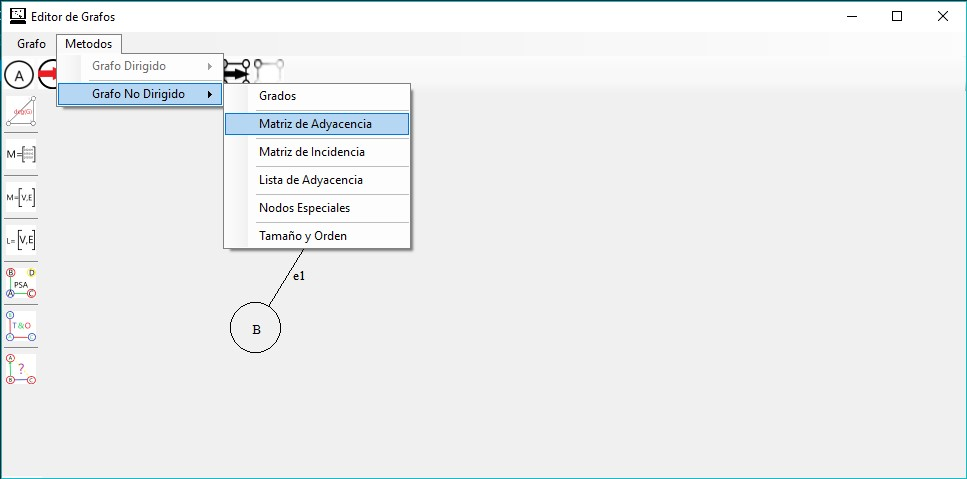
\includegraphics[scale=.60]{Imagen/5.jpg} 
\end{center}

\end{document}